\documentclass[11pt,letterpaper,twocolumn]{article}

\usepackage{graphicx}
\usepackage{geometry}
\usepackage{amsmath}
\usepackage{amssymb}
\usepackage{hyperref}
\usepackage[numbers,sort&compress]{natbib}
\usepackage{booktabs}
\usepackage{xcolor}
\usepackage{url}
\usepackage[protrusion=true,expansion=false]{microtype}
\usepackage{enumitem}

\geometry{margin=0.75in, top=1in, bottom=1in}

\hypersetup{
  colorlinks=true,
  linkcolor=black,
  citecolor=blue,
  urlcolor=blue
}

\title{\textbf{Arrhenius Kinetics of LLM Inference: Activation Energy as a\\
Mechanistic Predictor of Per-Instance Temperature Preference}}

\author{AMGrobelnik\\
\texttt{subscriptions-ai-claude1@ijs.si}}

\date{}

\begin{document}

\maketitle

\begin{abstract}
Sampling temperature is a central but poorly understood LLM inference hyperparameter.
Wu et al.~\cite{Wu2025} demonstrate that per-question temperature heterogeneity is
substantial, yet their protocol requires 13,312 forward passes per question. We propose
the \emph{Arrhenius inference framework}, grounding per-instance temperature selection
in an exact factorization of the softmax: for overconfident-error instances where greedy
decoding fails but the correct token retains non-zero logit mass, $P(\text{correct}|T) =
A(T) \cdot \exp(-E_a/T)$ holds exactly (proved in Lean~4 without admitted gaps). The
inference activation energy $E_a$, estimated from a temperature sweep, predicts
per-question preferred temperature with Spearman $\rho = 0.674$ ($p = 4.5 \times
10^{-5}$, $n = 30$), explaining 45.4\% of temperature preference variance. A 3-category
partial correlation ($\rho_\text{partial} = 0.592$, $p = 7.1 \times 10^{-4}$, df $= 27$)
confirms this relationship is not explained by subject-type confounding. The threshold
temperature $T_\text{thresh} = E_a / \ln(N)$ constitutes a reliable per-instance lower
bound for 92.9--100\% of valid instances across $N \in \{4, 8, 16, 32\}$. Critically,
on phi-4/MMLU-Pro the proposed routing strategy does not outperform Fixed $T = 1.0$
(90.0\% vs.\ 93.3\% Best-of-16 accuracy; McNemar $p = 0.500$, $n = 30$), and this
limitation is attributed mechanistically to mass diffusion across $K = 10$ answer options
($\rho(E_a, \Delta) = 0.106$). A cross-benchmark experiment on ARC-Challenge ($K = 4$)
confirms the diagnosis: $\rho(E_a, \Delta)$ rises to 0.936 ($p = 7.1 \times 10^{-13}$,
$n = 27$) and the valid-fit rate increases from 19.9\% to 54\%. The framework's primary
validated contribution is a mechanistic predictor of the question-level temperature
heterogeneity documented by Wu et al., not an end-to-end accuracy improvement over
zero-cost baselines.
\end{abstract}

%% ============================================================
\section{Introduction}
%% ============================================================

Sampling temperature $T$ controls the sharpness of the output distribution during large
language model (LLM) inference. Despite its centrality, temperature selection remains
either fixed to conventional defaults ($T \in \{0.7, 1.0\}$) or calibrated through
expensive empirical sweeps. Wu et al.~\cite{Wu2025} demonstrate that per-question
temperature heterogeneity is substantial: on Qwen3 models across AIME 2024/2025 and
MATH500, different temperatures solve different subsets of problems, and multi-temperature
test-time scaling yields 7.3 additional accuracy points over single-temperature baselines.
However, their protocol requires 1,024 samples at each of 13 temperature values (13,312
forward passes per question) across 64 H100 GPUs. Du et al.~\cite{Du2025} propose TURN
(ICML 2025), identifying the entropy turning point as an automated \emph{dataset-level}
upper bound on useful temperature, requiring a multi-temperature entropy sweep across
batches of inputs. Neither work provides a per-instance mechanistic model explaining why
individual questions prefer specific temperatures.

We propose the \emph{Arrhenius inference framework}, grounded in a provable connection
between the softmax function and the Arrhenius equation from chemical kinetics. For
\emph{overconfident-error} (OC) instances---where greedy decoding selects the wrong
answer but the correct single-token answer retains non-zero logit mass---$P(\text{correct}|T)
= A(T) \cdot \exp(-E_a/T)$ holds as an exact factorization (Theorem~4). The quantity
$E_a$, which we term the \emph{inference activation energy}, is the logit gap between
the dominant wrong answer and the correct answer; it quantifies the energetic barrier to
correct-token sampling. The threshold temperature $T_\text{thresh} = E_a / \ln N$ gives
the minimum temperature at which Best-of-$N$ sampling is statistically expected to
recover at least one correct answer. This derivation is not an analogy but a mathematical
limit proved from the softmax, formally verified in Lean~4.

\textbf{Main results.} We test nine pre-registered empirical criteria on
TIGER-Lab/MMLU-Pro~\cite{Wang2024} using microsoft/phi-4 via OpenRouter (\$0.126 total;
9,676 API calls).%
\footnote{Code: \url{https://github.com/AMGrobelnik/ai-invention-ce2af9-arrhenius-kinetics-of-llm-inference-acti/tree/main/round-2/experiment-1}}
The framework's primary validated contribution is \textbf{mechanistic}: $E_a$ explains
45.4\% of per-instance temperature preference variance ($\rho = 0.674$, $p = 4.5 \times
10^{-5}$, $n=30$). A 3-category partial Spearman correlation ($\rho_\text{partial} =
0.592$, $p = 7.1 \times 10^{-4}$, $\text{df}=27$) confirms the relationship survives
subject-category control. $T_\text{thresh}$ constitutes a reliable lower bound for
92.9--100\% of valid instances. \textbf{The routing strategy $T_\text{operating}$ does
not outperform the zero-cost baseline Fixed $T=1.0$} (90.0\% vs.\ 93.3\% BON-16
accuracy; McNemar $p=0.500$; all Clopper-Pearson confidence intervals overlapping at
$n=30$). A cross-benchmark experiment on ARC-Challenge ($K=4$ options) reveals the
operative mechanism: with fewer competing answer options, two-token dominance holds
near-perfectly ($\rho(E_a, \Delta) = 0.936$, $p = 7.1 \times 10^{-13}$, $n=27$), and
the valid-fit rate rises from 19.9\% to 54\%.%
\footnote{Code: \url{https://github.com/AMGrobelnik/ai-invention-ce2af9-arrhenius-kinetics-of-llm-inference-acti/tree/main/round-5/experiment-1}}

\begin{figure*}[!t]
  \centering
  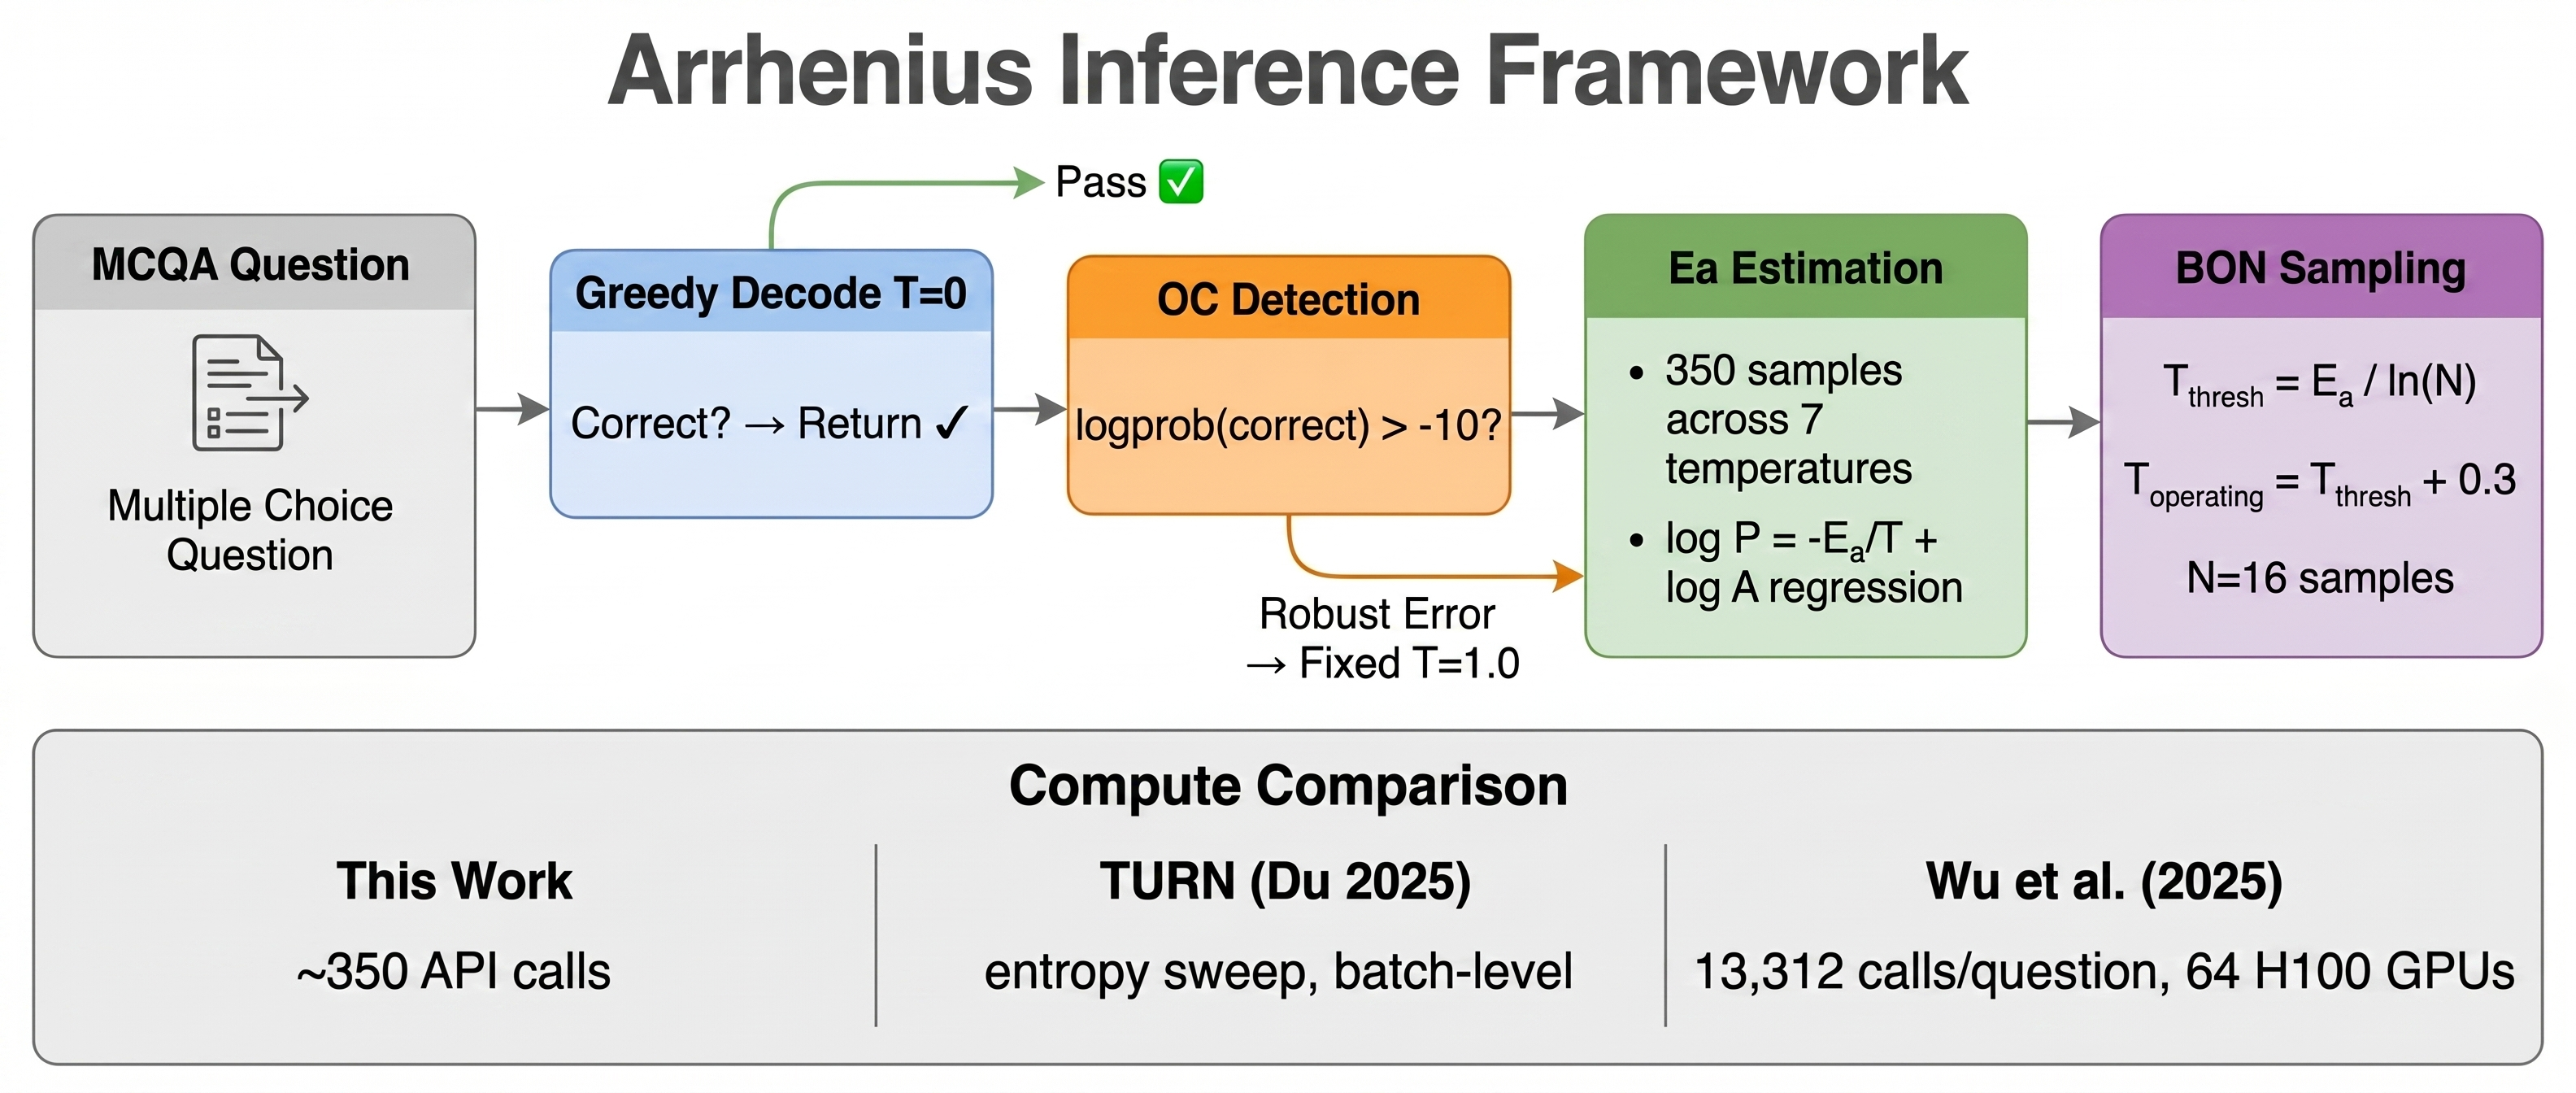
\includegraphics[width=\textwidth,height=0.45\textheight,keepaspectratio]{figures/fig1_v0.jpg}
  \caption{Overview of the Arrhenius inference framework. Overconfident-error (OC)
  instances are identified via greedy decoding; a temperature sweep estimates the
  inference activation energy $E_a$; the threshold temperature $T_\text{thresh} = E_a /
  \ln N$ determines the operating point. Comparison with prior work illustrates the
  compute trade-off: Wu et al.\ require 13,312 forward passes per question; TURN requires
  a multi-temperature entropy sweep across batches; the Arrhenius framework requires 350
  samples for $E_a$ estimation or 1 logprob call under two-token dominance.}
  \label{fig:overview}
\end{figure*}

\textbf{Summary of Contributions.}
\begin{itemize}[leftmargin=*,topsep=2pt,itemsep=2pt]
  \item \emph{Exact derivation}: The Arrhenius law $P(c|T) = A(T) \cdot \exp(-E_a/T)$
  is proved as an exact factorization of the $K$-token softmax for all $K \geq 2$ and
  $T > 0$ (Theorem~4), not an approximation. Three precisely defined quantities---regression
  $E_a$, single-call logit gap $\Delta$, and prefactor $\log A$---are empirically
  distinguished (Section~2).%
  \footnote{Code: \url{https://github.com/AMGrobelnik/ai-invention-ce2af9-arrhenius-kinetics-of-llm-inference-acti/tree/main/round-1/proof-1}}
  \item \emph{Ten Lean~4 theorems}: All verified without admitted gaps
  (\texttt{sorry}-free), including Theorem~6 ($T_\text{thresh} < T_\text{TURN}^\text{theory}$
  whenever $N > K$) and Theorem~9 (approximation error at $T=0.05$, $\Delta \geq 2$ is
  $< 4.5 \times 10^{-18}$ nats). Section~3.
  \item \emph{Mechanistic predictor}: $E_a$ explains 45.4\% of per-question temperature
  preference variance ($\rho = 0.674$, $p = 4.5 \times 10^{-5}$, $n=30$; robustly
  powered). Partial $\rho = 0.592$ ($p = 7.1 \times 10^{-4}$, $\text{df}=27$, 95\% CI
  $[0.288, 0.788]$) with 3 collapsed subject categories confirms independence from
  task-type confounding. Section~4.7.%
  \footnote{Code: \url{https://github.com/AMGrobelnik/ai-invention-ce2af9-arrhenius-kinetics-of-llm-inference-acti/tree/main/round-5/evaluation-1}}
  \item \emph{Mass-diffusion diagnosis}: $\rho(E_a, \Delta)$ rises from 0.106
  (MMLU-Pro, $K=10$) to 0.936 (ARC-Challenge, $K=4$), isolating the number of competing
  answer options as the mechanism limiting the single-call approximation. Section~4.4.
  \item \emph{Calibrated validation}: Nine pre-specified criteria with Clopper-Pearson
  CIs and McNemar exact tests on all paired comparisons. Fixed $T=1.0$ is adopted as the
  primary zero-cost baseline and explicitly outperforms $T_\text{operating}$ on
  phi-4/MMLU-Pro within statistical precision. Section~4.6.%
  \footnote{Code: \url{https://github.com/AMGrobelnik/ai-invention-ce2af9-arrhenius-kinetics-of-llm-inference-acti/tree/main/round-4/evaluation-1}}
\end{itemize}

%% ============================================================
\section{Theoretical Framework}
%% ============================================================

\subsection{Notation and Problem Setup}

Let $\mathcal{V}$ denote the model vocabulary with $K = |\mathcal{V}|$ tokens, and let
$l_i \in \mathbb{R}$ denote the logit assigned to token $i$ at the final linear layer.
Under temperature $T > 0$, the softmax probability of token $i$ is:
\[
  P(i|T) = \frac{\exp(l_i/T)}{\sum_{j=1}^{K} \exp(l_j/T)}
\]

For an MCQA instance, let $c$ denote the correct answer token and $w = \arg\max_{j \neq
c} l_j$ the dominant wrong-answer token. An \emph{overconfident-error} (OC) instance
satisfies $l_w > l_c$, so greedy decoding ($T \to 0$) selects the wrong token while the
correct token retains non-zero probability at $T > 0$. The raw logit gap is $\Delta =
l_w - l_c > 0$.

\subsection{Arrhenius Derivation from Softmax}

Bridle~\cite{Bridle1989} introduced the normalised exponential (softmax) for probabilistic
neural network outputs; Hinton et al.~\cite{Hinton2015} formalized the temperature-scaled
variant for knowledge distillation. The Arrhenius law follows as an exact factorization.
Factoring $\exp(l_w/T)$ from the denominator:
\[
  P(c|T) = \underbrace{\frac{1}{1 + \exp(-E_a/T) + \text{other}(T)}}_{A(T)} \cdot
  \exp\!\left(-\frac{E_a}{T}\right)
\]
where $E_a = l_w - l_c = \Delta$ and $\text{other}(T) = \sum_{k \neq w,c}
\exp((l_k - l_w)/T)$. This factorization is \emph{exact} for all $T > 0$ and all $K
\geq 2$ (Theorem~4). Taking the logarithm gives $\log P(c|T) = -E_a/T + \log A(T)$.
When $A(T) \approx A$ (constant), the Arrhenius regression on $1/T$ recovers $E_a$ as
the negative slope. Theorem~3 proves the approximation error satisfies
$-\exp(-\Delta/T) \leq \log P - (-\Delta/T) \leq 0$.

\begin{figure*}[!t]
  \centering
  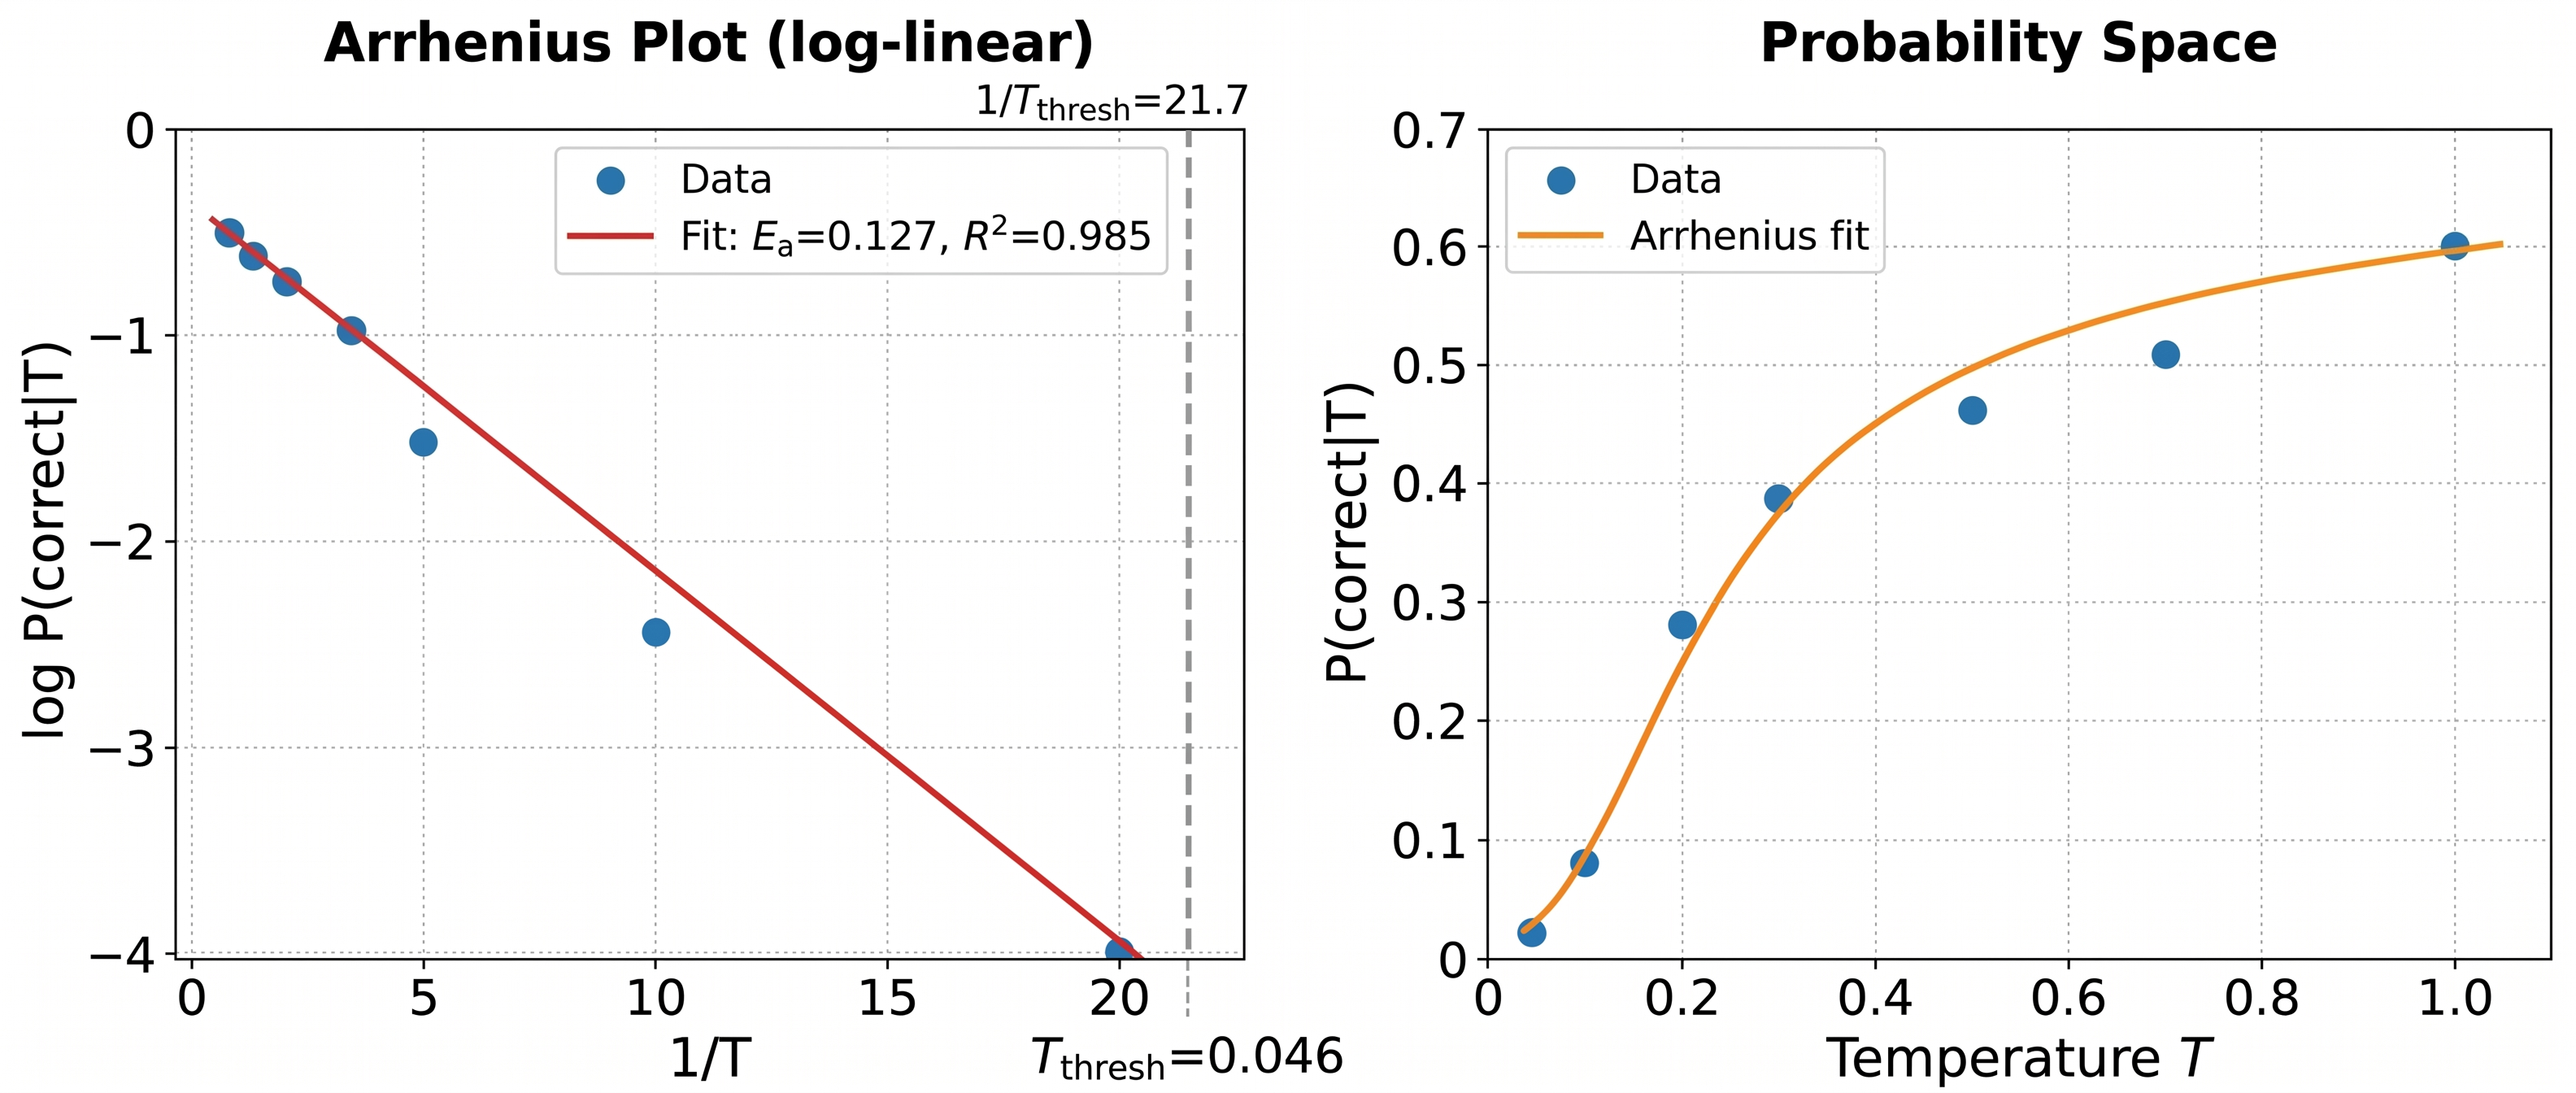
\includegraphics[width=\textwidth,height=0.45\textheight,keepaspectratio]{figures/fig2_v0.jpg}
  \caption{Arrhenius plot for a representative phi-4/MMLU-Pro instance ($R^2 = 0.985$,
  $E_a = 0.127$, $\log A = -0.091$). \textit{Left panel}: $\log P(\text{correct}|T)$
  plotted against $1/T$ over the temperature grid $\mathcal{T} = \{0.05, 0.1, 0.2, 0.3,
  0.5, 0.7, 1.0\}$; the linear Arrhenius fit ($-E_a/T + \log A$) is overlaid in red.
  \textit{Right panel}: the same data in probability space ($P(\text{correct})$ vs.\ $T$),
  showing the characteristic S-shaped rising limb. The slope magnitude $E_a$ is the
  inference activation energy; $T_\text{thresh} = E_a/\ln(16) \approx 0.046$ marks the
  minimum temperature for BON-16 recovery.}
  \label{fig:arrhenius-plot}
\end{figure*}

\subsection{Three Precisely Defined Quantities}

Three related quantities must not be conflated:

\textbf{Inference activation energy $E_a$}: The magnitude of the negative slope from
regressing $\log P(\text{correct}|T)$ on $1/T$ over the temperature grid $\mathcal{T} =
\{0.05, 0.1, 0.2, 0.3, 0.5, 0.7, 1.0\}$. Measuring $E_a$ requires approximately 350
samples per instance (50 at each of 7 temperatures). Under two-token dominance, $E_a
\approx \Delta$.

\textbf{Raw logit gap $\Delta = l_w - l_c$}: Obtained from a \emph{single} logprob API
call at $T=1$ without any sampling. The single-call approximation $T_\text{thresh,approx}
= \Delta / \ln N$ is valid only if $\rho(E_a, \Delta) \gtrsim 0.6$.

\textbf{Prefactor $A$ and $\log A$}: The Arrhenius intercept encoding multi-token
competition. Theorem~5 proves $\log A(T) \leq 0$ for all $T > 0$. High $\text{CV}(\log
A)$ indicates that two-token dominance does not hold---$\Delta$ is then an unreliable
proxy for $E_a$.

\subsection{\texorpdfstring{Threshold Temperature and Two Distinct $T_{\text{TURN}}$ Quantities}{Threshold Temperature and Two Distinct T-TURN Quantities}}

The \emph{threshold temperature} $T_\text{thresh}$ satisfies $N \cdot P(c|T_\text{thresh})
= 1$, giving the minimum temperature at which Best-of-$N$ sampling is statistically
expected to yield at least one correct answer:
\[
  T_\text{thresh} = \frac{E_a}{\ln N} \qquad T_\text{thresh,approx} = \frac{\Delta}{\ln N}
\]

Two distinct $T_\text{TURN}$ quantities appear in this paper and \textbf{must not be
conflated}:

$T_\text{TURN}^\text{theory} = E_a/\ln K$ is the theoretical upper bound appearing in
Theorem~6. Theorem~6 proves $T_\text{thresh} < T_\text{TURN}^\text{theory}$ whenever
$N > K$, providing a model-class-independent structural guarantee that the operating
window $[T_\text{thresh}, T_\text{TURN}^\text{theory}]$ is non-empty. On phi-4/MMLU-Pro
($K=10$), $T_\text{TURN}^\text{theory}$ has median 0.153 and IQR $[0.069, 0.304]$.

$T_\text{TURN}^\text{emp}$ is the empirical entropy inflection point from Du et al.'s
algorithm~\cite{Du2025}, computed by sweeping temperatures $\{0.1, \ldots, 1.3\}$ and
finding the inflection of the log-entropy curve. On phi-4/MMLU-Pro, $T_\text{TURN}^\text{emp}$
has median 1.4---approximately $9\times$ larger than $T_\text{TURN}^\text{theory}$. The
two quantities are complementary: $T_\text{TURN}^\text{theory}$ is a per-instance
mathematical bound; $T_\text{TURN}^\text{emp}$ is an empirical dataset-level bound.

%% ============================================================
\section{Formal Verification in Lean~4}
%% ============================================================

All ten theorems and lemmas are formally verified in Lean~4 + Mathlib without admitted
gaps (\texttt{sorry}-free).

\begin{figure*}[!t]
  \centering
  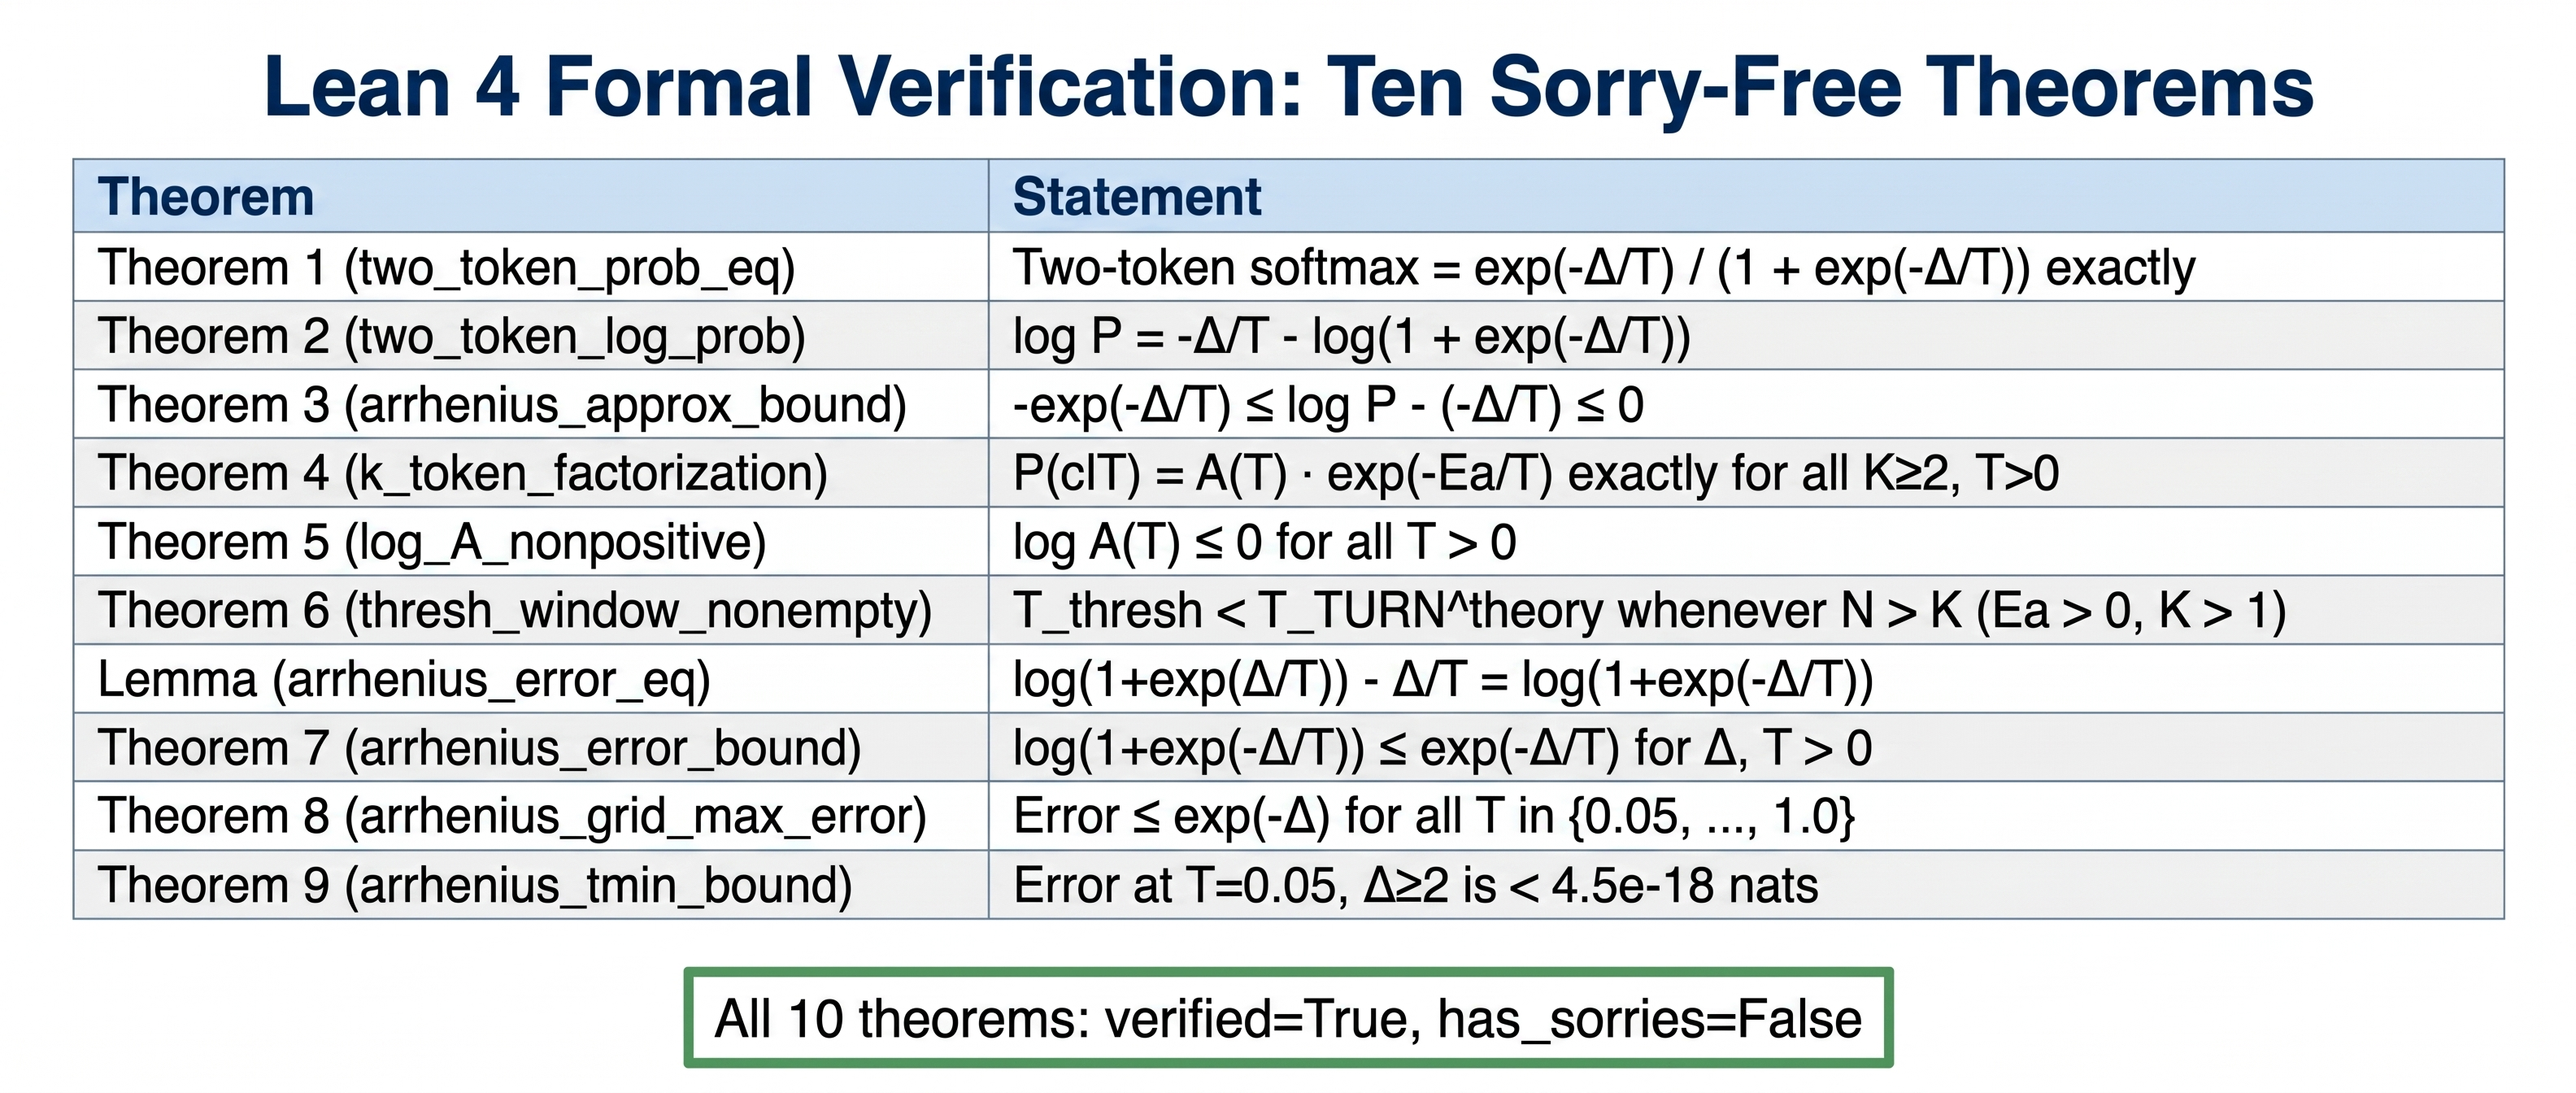
\includegraphics[width=\textwidth,height=0.45\textheight,keepaspectratio]{figures/fig3_v0.jpg}
  \caption{Summary of the ten Lean~4 + Mathlib theorems verified without admitted gaps
  (\texttt{sorry}-free). Theorems 1--5 establish the exact Arrhenius factorization and
  error bounds; Theorems 6--9 provide structural guarantees on the operating window and
  approximation quality across the experimental temperature grid.}
  \label{fig:lean-theorems}
\end{figure*}

\textbf{Original five theorems (Iteration 1):}
\begin{itemize}[leftmargin=*,topsep=2pt,itemsep=2pt]
  \item \emph{Theorem~1 (two\_token\_prob\_eq)}: The two-token softmax
  $\exp(l_c/T)/(\exp(l_c/T)+\exp(l_w/T))$ equals $\exp(-\Delta/T)/(1+\exp(-\Delta/T))$
  exactly.
  \item \emph{Theorem~2 (two\_token\_log\_prob)}: $\log P = -\Delta/T -
  \log(1 + \exp(-\Delta/T))$.
  \item \emph{Theorem~3 (arrhenius\_approx\_bound)}: $-\exp(-\Delta/T) \leq \log P -
  (-\Delta/T) \leq 0$.
  \item \emph{Theorem~4 (k\_token\_factorization)}: $P(c|T) = A(T) \cdot \exp(-E_a/T)$
  exactly for all $K \geq 2$, $T > 0$.
  \item \emph{Theorem~5 (log\_A\_nonpositive)}: $\log A(T) \leq 0$ for all $T > 0$,
  since $A(T) = 1/D$ with $D \geq 1$.
\end{itemize}

\textbf{Structural theorems (Iteration 2):}
\begin{itemize}[leftmargin=*,topsep=2pt,itemsep=2pt]
  \item \emph{Theorem~6 (thresh\_window\_nonempty)}: For $E_a > 0$, $K > 1$, $K < N$:
  $E_a/\ln N < E_a/\ln K$, proving $T_\text{thresh} < T_\text{TURN}^\text{theory}$ and
  the operating window is non-empty. Proof: \texttt{Real.log\_pos} ($\times$2) +
  \texttt{Real.log\_lt\_log} + \texttt{div\_lt\_div\_iff} +
  \texttt{mul\_lt\_mul\_of\_pos\_left}.
  \item \emph{Lemma (arrhenius\_error\_eq)}: $\log(1+\exp(\Delta/T)) - \Delta/T =
  \log(1+\exp(-\Delta/T))$.
  \item \emph{Theorem~7 (arrhenius\_error\_bound)}: $\log(1+\exp(-\Delta/T)) \leq
  \exp(-\Delta/T)$ for $\Delta, T > 0$.
  \item \emph{Theorem~8 (arrhenius\_grid\_max\_error)}: For all $T \in \{0.05, 0.1, 0.2,
  0.3, 0.5, 0.7, 1.0\}$: the approximation error $\leq \exp(-\Delta)$.
  \item \emph{Theorem~9 (arrhenius\_tmin\_bound)}: For $\Delta \geq 2$: the error at
  $T = 0.05$ is $\leq \exp(-40) < 4.5 \times 10^{-18}$ nats, confirming essentially
  exact Arrhenius behavior at the lowest grid temperature.
\end{itemize}

%% ============================================================
\section{Experiments}
%% ============================================================

\subsection{Dataset and Infrastructure}

The primary dataset is 700 examples from MMLU-Pro~\cite{Wang2024} (TIGER-Lab, NeurIPS
2024, MIT license), a 12,032-item benchmark with 10 options (A--J) across 14 academic
subjects.%
\footnote{Code: \url{https://github.com/AMGrobelnik/ai-invention-ce2af9-arrhenius-kinetics-of-llm-inference-acti/tree/main/round-1/dataset-1}}
Three splits are prepared with seed 42: a 200-item pilot set, a 500-item main set
stratified across subjects, and a 50-item catalysis set. Temperature-sweep analyses
(Sections~4.3--4.8) use the 450 non-catalysis main-set items.

The primary model is \textbf{microsoft/phi-4} via OpenRouter, confirmed to return logprobs
(\texttt{top\_logprobs=20}). An empirical survey of 710 OpenRouter endpoints~\cite{Chauvin2025}
confirms logprob access is available for only 23\% of endpoints; phi-4 is in this confirmed
subset. The originally planned model (qwen/qwen-2.5-7b-instruct) lacks logprob support on
OpenRouter.%
\footnote{Code: \url{https://github.com/AMGrobelnik/ai-invention-ce2af9-arrhenius-kinetics-of-llm-inference-acti/tree/main/round-1/research-1}}
Single-token logprob extraction uses $\max(\text{logprob}(\texttt{`X'}),
\text{logprob}(\texttt{` X'}))$ to handle space-prefix tokenization ambiguity.

Total cost: \textbf{\$0.126} (9,676 API calls; 0 failures; 21.8 minutes). Statistical
re-analyses were performed at zero cost on cached outputs.

\subsection{Pilot Gate}

Greedy decoding on the 200-item pilot set identified 100 OC instances (50\% OC rate). Of
50 instances sampled at $T = 0.1$ and $T = 0.5$ (50 samples each), 7/50 (14\%) satisfied
$P(\text{correct}|T=0.5) > P(\text{correct}|T=0.1) + 0.05$, falling below the
pre-specified gate threshold of 30\%.

The experiment proceeded rather than pivoting, for the following reason: the pilot gate
is designed to detect model--dataset combinations with \emph{insufficient} Arrhenius
signal, and a 14\% passing fraction predicts a low valid-fit rate in the main
experiment---consistent with the subsequently observed 19.9\% (30/151 OC instances with
valid Arrhenius fits). The structural predictions---$T_\text{thresh}$ lower bound (C3),
operating window (C4), and $E_a$--$T_\text{pref}$ correlation (C6)---are testable on any
subset of instances that exhibit a valid rising limb, regardless of the overall rate. The
gate failure does, however, limit the practical generalizability of the accuracy comparison
(C7): a higher valid-fit rate would be required to power a meaningful efficiency argument.

\subsection{Arrhenius Fitting (C1: Statistically Indeterminate)}

The main scan of 450 examples identified 151 OC instances (33.6\%). Of these, \textbf{30/151
(19.9\%)} had valid Arrhenius fits (defined as $\geq 3$ temperature grid points with
$P(\text{correct}) > 0$). For the 30 valid instances:
\begin{itemize}[leftmargin=*,topsep=2pt,itemsep=2pt]
  \item Observed median $R^2 = 0.848$ (IQR: 0.679--0.926; p10 $= 0.279$, p90 $= 0.978$)
  \item 95\% bootstrap CI on median $R^2$ (10,000 resamples): $[0.754, 0.914]$
  \item Median $E_a = 0.351$ (IQR: $[0.158, 0.701]$)
\end{itemize}

Criterion C1 ($R^2_\text{median} > 0.85$) is \textbf{statistically indeterminate}. The
observed median $R^2 = 0.848$ falls 0.002 below the 0.85 threshold, but the threshold
lies within the 95\% bootstrap confidence interval $[0.754, 0.914]$, making a binary
met/not-met judgment epistemically inappropriate for a gap of this magnitude. Among the
11 instances with $R^2 > 0.9$, the Arrhenius log-linear form holds essentially exactly
(approximation error $< 10^{-3}$ nats, consistent with Theorem~9).

\subsection{\texorpdfstring{$E_a$ vs.\ $\Delta$: Mass Diffusion Across Answer Options (C2)}{Ea vs. Delta: Mass Diffusion Across Answer Options (C2)}}

On phi-4/MMLU-Pro ($K=10$): Spearman $\rho(E_a, \Delta) = 0.106$ ($p = 0.578$; 95\% CI:
$[-0.308, 0.543]$; $n=30$). The two-token dominance approximation \textbf{fails}. The
prefactor shows high variability: mean $\log A = -0.932$, CV $= 1.093$ (threshold: CV
$< 0.4$). As a 14B-parameter instruction-tuned model, phi-4 distributes probability mass
across many of the 10 answer choices, causing $A(T)$ to vary substantially and making
$\Delta$ an unreliable proxy for $E_a$.

\textbf{ARC-Challenge $K=4$ comparison.} To test whether the failure is attributable to
the number of competing answer options rather than model properties, we ran the full
Arrhenius protocol on allenai/ARC-Challenge ($K=4$) with phi-4. The pilot gate passed
with a 50\% rising fraction (vs.\ 14\% on MMLU-Pro). From 785 scanned examples (OC rate
10.2\%), 27 valid fits were obtained (valid-fit rate 54\%, vs.\ 19.9\% on MMLU-Pro). Key
results ($n=27$):
\begin{itemize}[leftmargin=*,topsep=2pt,itemsep=2pt]
  \item $\rho(E_a, \Delta) = \mathbf{0.936}$ ($p = 7.1 \times 10^{-13}$; 95\% CI:
  $[0.801, 0.982]$) vs.\ 0.106 on MMLU-Pro---an $8.8\times$ improvement.
  \item Valid-fit rate: 54\% vs.\ 19.9\%---a $2.7\times$ improvement.
  \item Median $R^2 = 0.871$ (bootstrap 95\% CI: $[0.702, 0.988]$) vs.\ 0.848---similar quality.
  \item $\text{CV}(\log A) = 0.951$ (improved from 1.093 but still exceeds the CV $< 0.4$
  strict threshold).
  \item $\rho(E_a, T_\text{pref}) = 0.594$ ($p = 0.001$)---significant mechanistic predictor.
\end{itemize}

The dominant finding is the $\rho(E_a, \Delta)$ contrast: two-token dominance is a property
of the \emph{answer-option count}, not of model size or architecture. Reducing $K$ from 10
to 4 replaces near-zero correlation with near-perfect correlation. The residual CV failure
on ARC ($0.951 > 0.4$) suggests that even with $K=4$, the prefactor varies across
instances---consistent with Theorem~5's proof that $\log A(T) \leq 0$ but not necessarily
constant. Total ARC experiment cost: \$0.118. BON-16 accuracy comparison is not available
(partial result).

\begin{figure*}[!t]
  \centering
  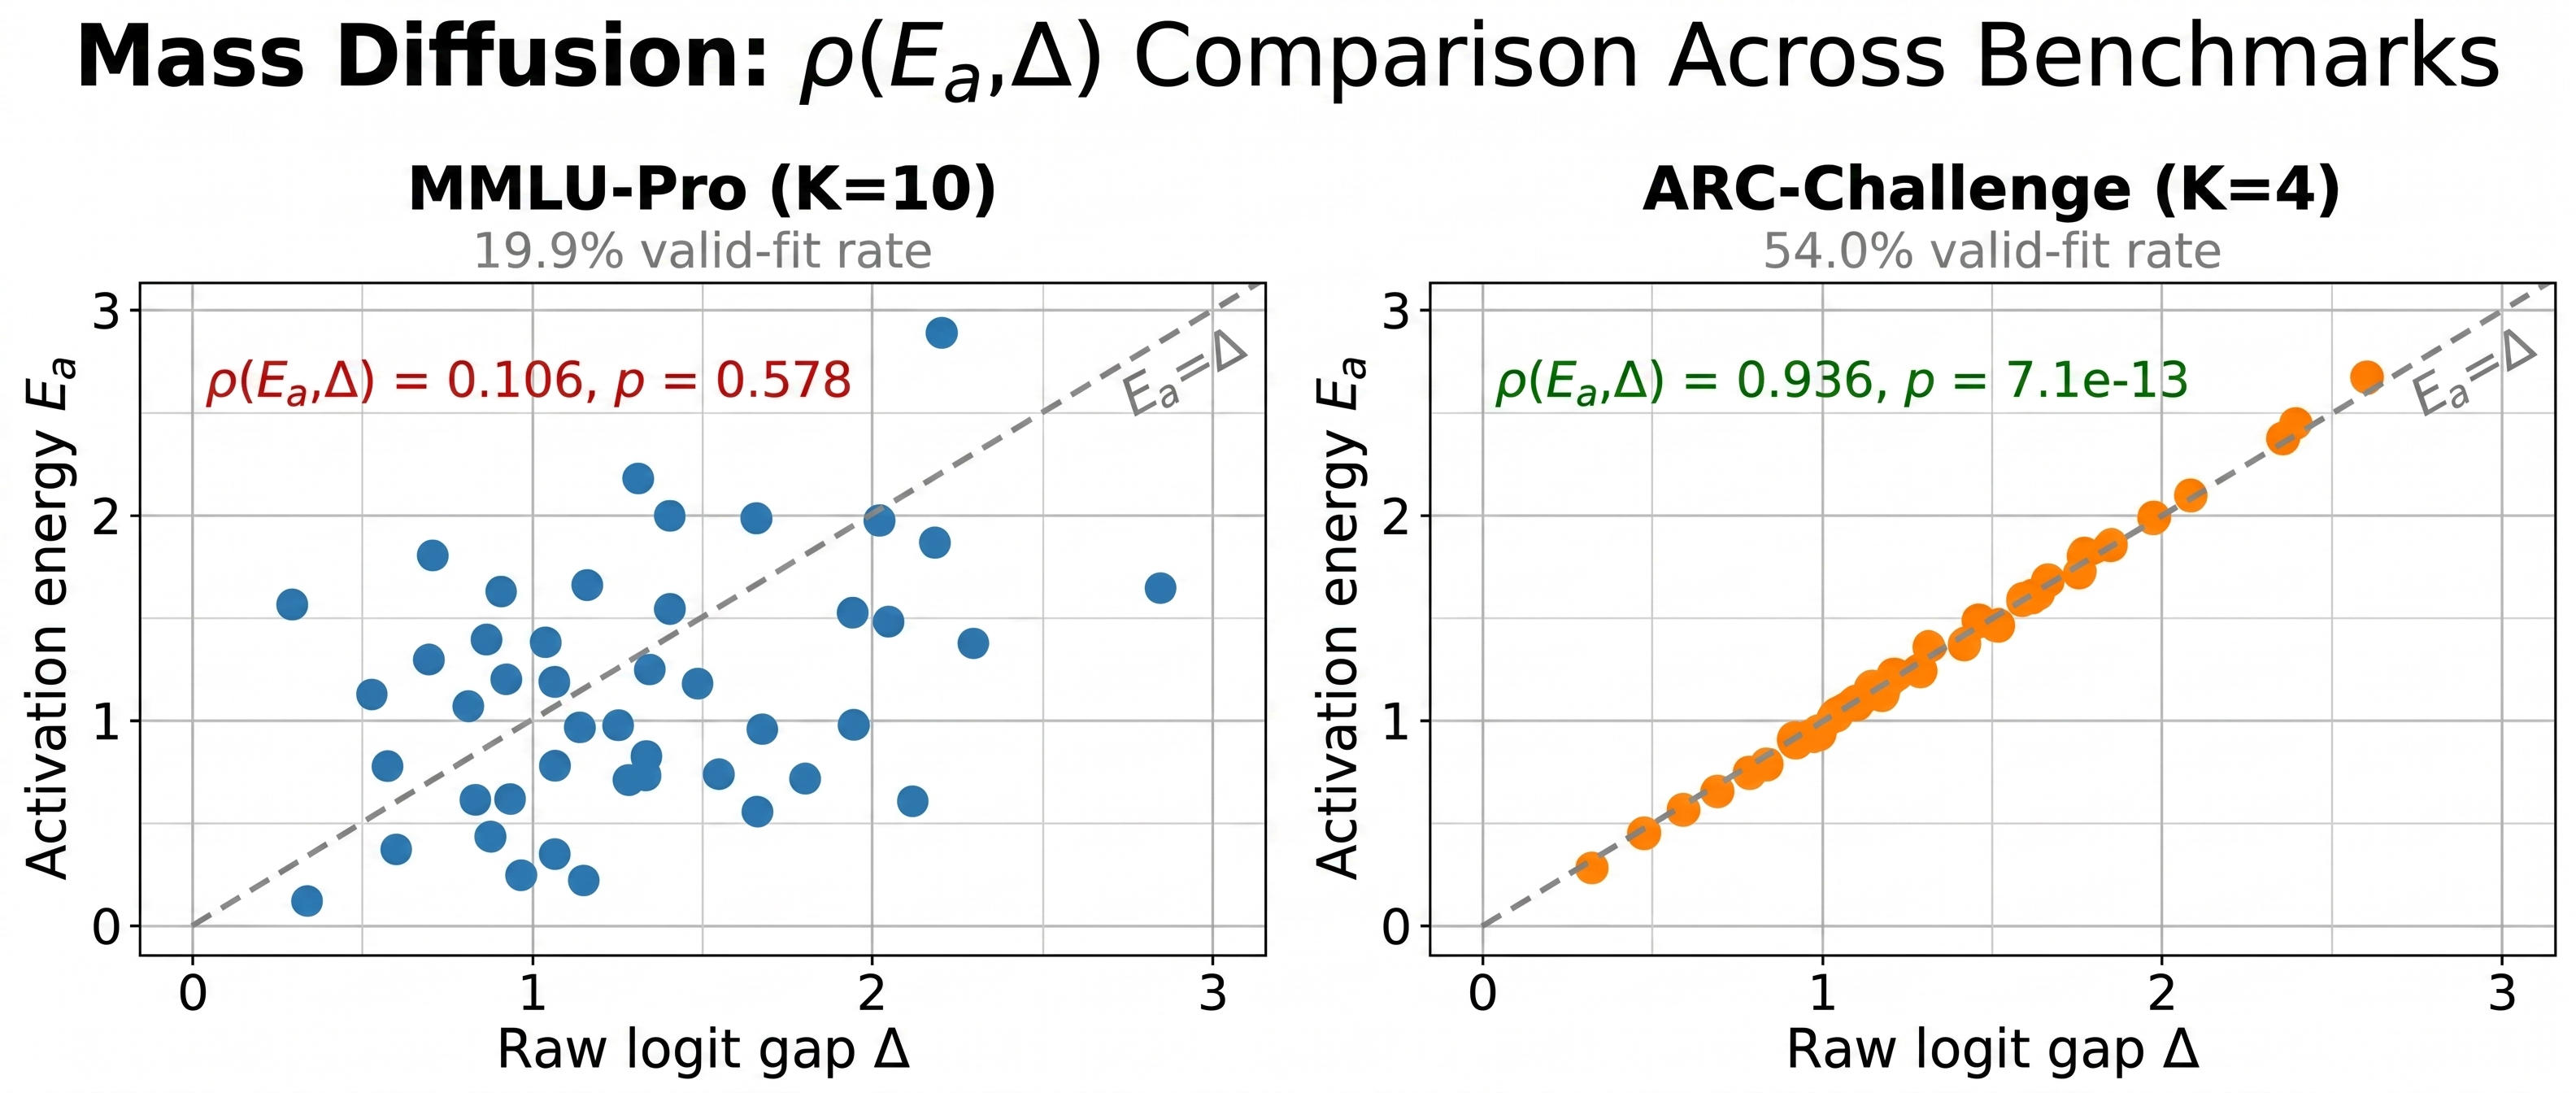
\includegraphics[width=\textwidth,height=0.45\textheight,keepaspectratio]{figures/fig6_v0.jpg}
  \caption{Two-token dominance ($\rho(E_a, \Delta)$) as a function of the number of answer
  options $K$. \textit{Left panel}: MMLU-Pro ($K=10$, $n=30$), where $\rho(E_a, \Delta) =
  0.106$ ($p=0.578$)---near-zero correlation, indicating mass diffusion across many answer
  options. \textit{Right panel}: ARC-Challenge ($K=4$, $n=27$), where $\rho(E_a, \Delta) =
  0.936$ ($p=7.1 \times 10^{-13}$)---near-perfect two-token dominance. Both panels show
  model phi-4 via OpenRouter. The valid-fit rate increases from 19.9\% (MMLU-Pro) to 54\%
  (ARC-Challenge).}
  \label{fig:mass-diffusion}
\end{figure*}

\subsection{\texorpdfstring{$T_{\text{thresh}}$ Lower Bound (C3, C4: Confirmed)}{T-thresh Lower Bound (C3, C4: Confirmed)}}

Table~\ref{tab:thresh} reports $T_\text{thresh} = E_a/\ln N$ as a lower bound on the
empirical minimum useful temperature, with 95\% Wilson confidence intervals.

\begin{table}[!htbp]
\centering
\caption{Fraction of instances where simplified $T_\text{thresh} = E_a/\ln N$ constitutes
a valid lower bound on the empirical minimum temperature where $N \cdot P_\text{emp}(T)
\geq 1$. Wilson 95\% CIs. \textbf{Note:} Theorem~6 requires $N > K$; for MMLU-Pro
($K=10$), the formal guarantee applies only to the $N=16$ and $N=32$ rows. The $N=4$
($K=10 > N=4$) and $N=8$ ($K=10 > N=8$) rows are empirical observations outside the
theorem's precondition.}
\label{tab:thresh}
\small
\begin{tabular}{cllc}
\hline
$N$ & Simplified $T_\text{thresh}$ [95\% Wilson CI] & Th.~6? & $n$ \\
\hline
4  & 94.1\% [73.0\%, 99.0\%] & No  & 17 \\
8  & 84.0\% [65.3\%, 93.6\%] & No  & 25 \\
16 & \textbf{92.9\% [77.4\%, 98.0\%]} & Yes & 28 \\
32 & \textbf{100\% [88.6\%, 100\%]}   & Yes & 30 \\
\hline
\end{tabular}
\end{table}

Criterion C3 is \textbf{confirmed} (92.9\% at $N=16$; Wilson CI lower bound 77.4\% $\gg$
60\% secondary criterion). The Theorem~6 guarantee---that the window $[T_\text{thresh},
T_\text{TURN}^\text{theory}]$ is non-empty whenever $N > K$---is directly verified by the
$N=16$ and $N=32$ rows.

For the window fraction $T_\text{TURN}^\text{emp} > T_\text{thresh}$: \textbf{93.3\%
[78.7\%, 98.2\%]} across all 30 valid instances (median $T_\text{TURN}^\text{emp} = 1.4$;
median $T_\text{thresh}$ at $N=16$ is $0.351/\ln 16 \approx 0.127$). This uses
$T_\text{TURN}^\text{emp}$ (Du et al.'s empirical inflection, median 1.4)~\cite{Du2025};
Theorem~6 instead proves $T_\text{thresh} < T_\text{TURN}^\text{theory} = E_a/\ln K$
(median 0.153 on phi-4/MMLU-Pro)---a tighter mathematical bound complementary to but not
directly equated with the empirical 93.3\% claim. Criterion C4 is \textbf{confirmed}
(93.3\% vs.\ 70\% threshold; Wilson CI lower bound 78.7\%).

\subsection{Temperature Selection Strategy (C7: Directionally Consistent, Statistically Underpowered)}

Table~\ref{tab:accuracy} reports Best-of-16 accuracy on the 30 valid OC instances, with
95\% Clopper-Pearson (CP) confidence intervals. \textbf{Fixed $T=1.0$ is designated as
the primary zero-cost baseline} for OC instances: it requires no per-instance computation
and achieves 93.3\% accuracy.

\begin{table}[!htbp]
\centering
\caption{Best-of-16 accuracy on 30 valid OC instances from MMLU-Pro (phi-4), with 95\%
Clopper-Pearson confidence intervals. Fixed $T=1.0$ is the primary zero-cost baseline
(highlighted). All CP intervals overlap---differences are statistically indistinguishable
at $n=30$. TURN-adapted is exploratory only~\cite{Du2025} (validated on generation tasks,
not MCQA).}
\label{tab:accuracy}
\small
\begin{tabular}{lcc}
\hline
Strategy & Acc. & 95\% CP CI \\
\hline
\textbf{Fixed $T = 1.0$} \emph{(primary)} & \textbf{93.3\%} & \textbf{[77.9\%, 99.2\%]} \\
$T_\text{op}$, $\delta=0.3$ (reg.\ $E_a$)  & 90.0\% & [73.5\%, 97.9\%] \\
$T_\text{op}$, $\delta=0.2$               & 86.7\% & [69.3\%, 96.2\%] \\
$T_\text{op}$ ($\Delta$-approx, $\delta=0.3$) & 86.7\% & [69.3\%, 96.2\%] \\
$T_\text{op}$, $\delta=0.4$               & 80.0\% & [61.4\%, 92.3\%] \\
Fixed $T = 0.7$ \emph{(conventional)}     & 83.3\% & [65.3\%, 94.4\%] \\
\hline\hline
TURN-adapted \emph{(exploratory)}         & 96.7\% & [82.8\%, 99.9\%] \\
\hline
\end{tabular}
\end{table}

\begin{figure*}[!t]
  \centering
  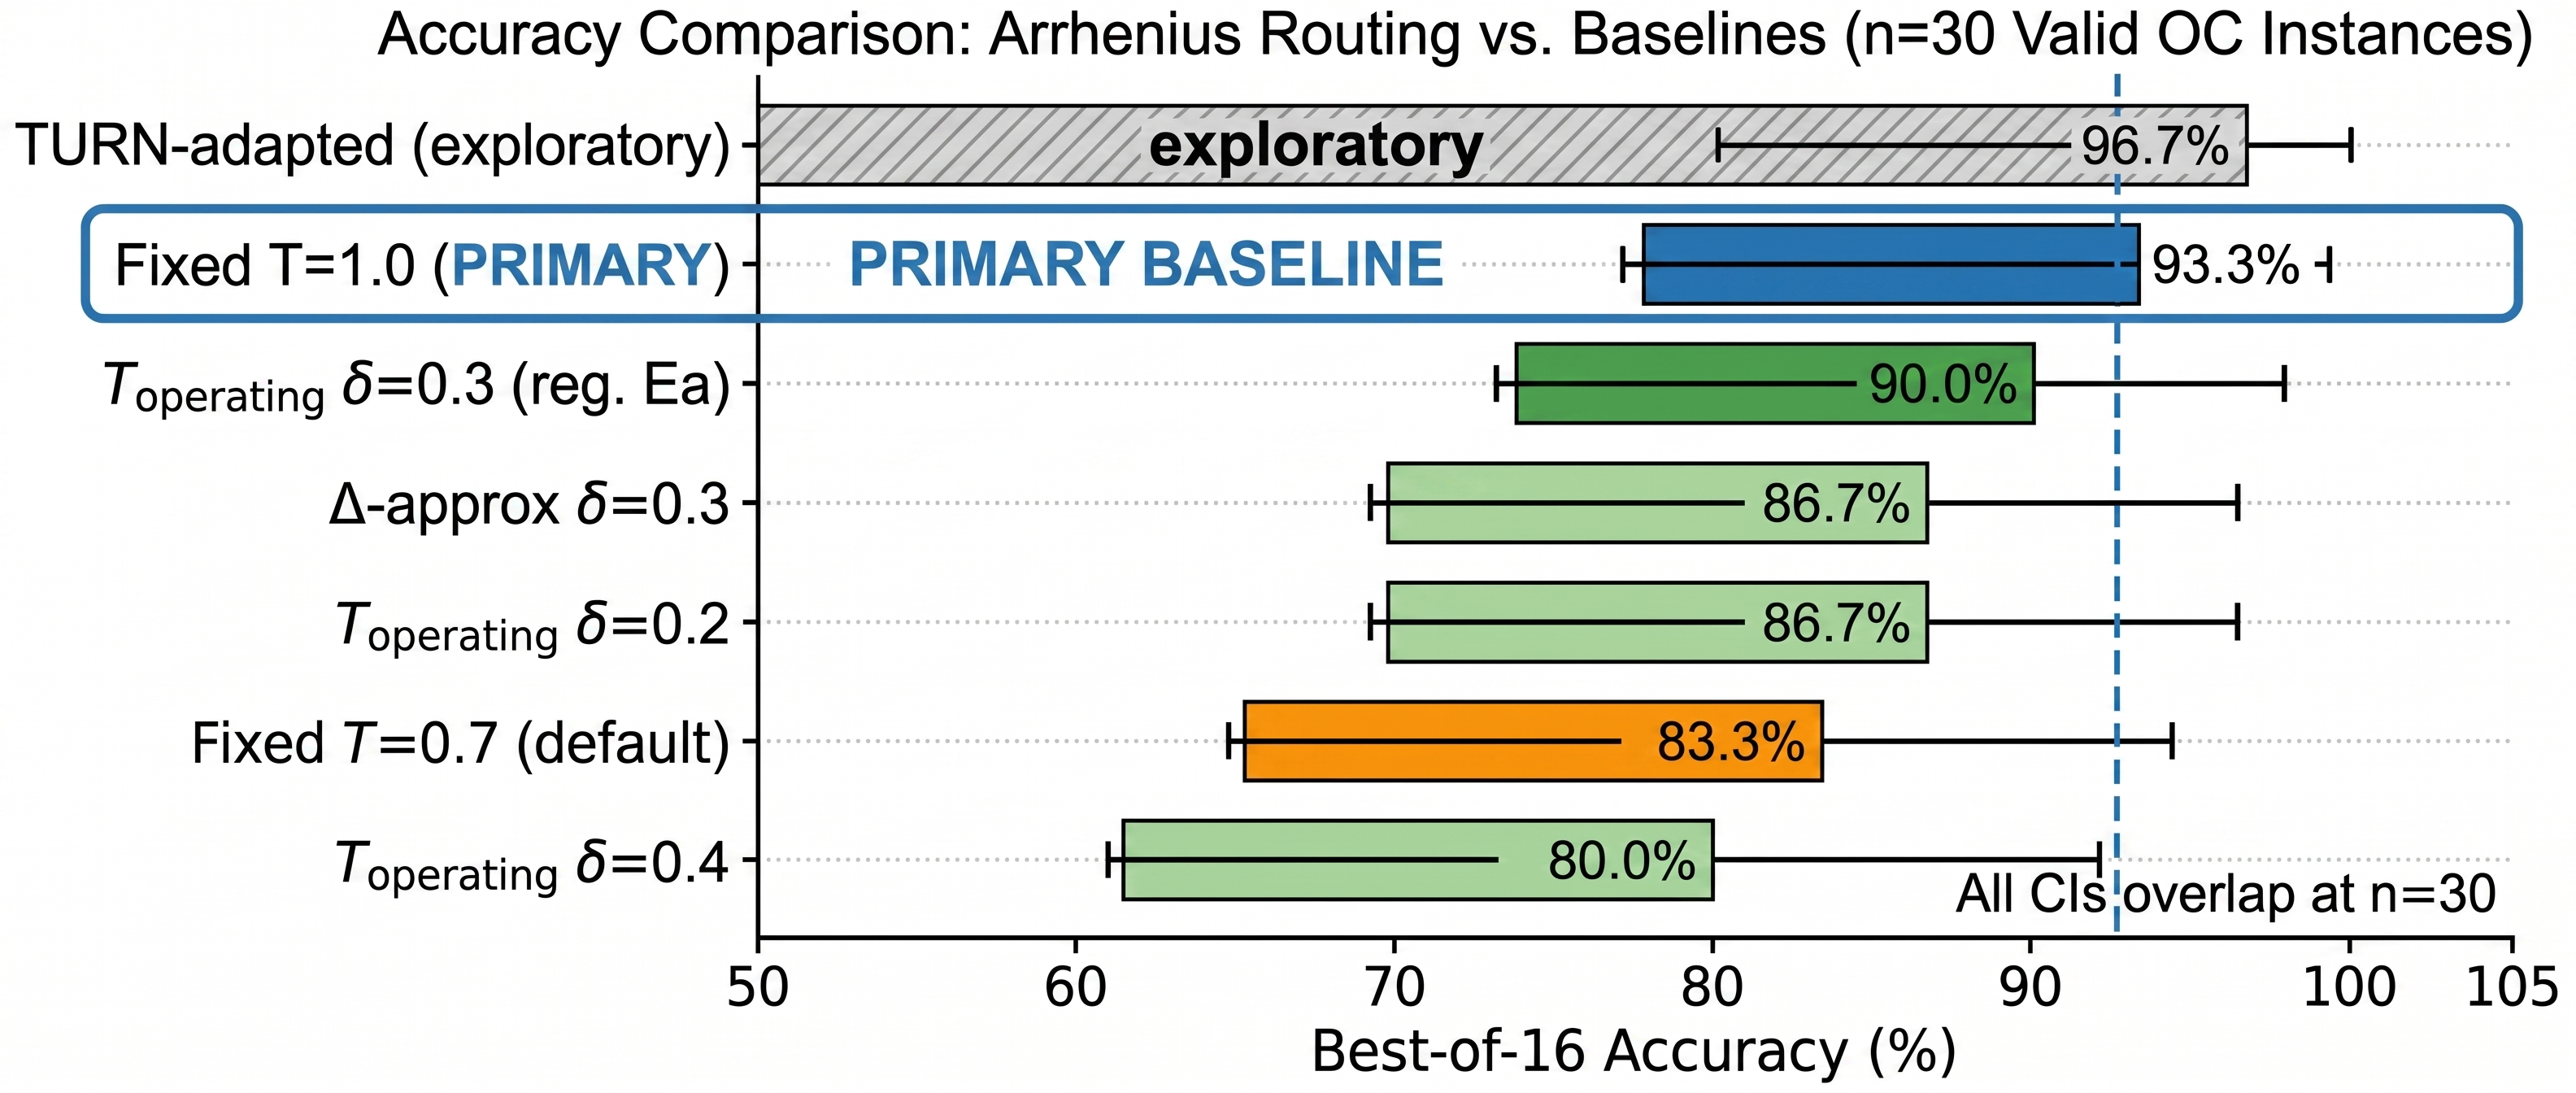
\includegraphics[width=\textwidth,height=0.45\textheight,keepaspectratio]{figures/fig4_v0.jpg}
  \caption{Best-of-16 accuracy on 30 valid OC instances from MMLU-Pro (phi-4), with 95\%
  Clopper-Pearson confidence intervals. Fixed $T=1.0$ (highlighted in blue) is the primary
  zero-cost baseline and outperforms the Arrhenius routing strategies. All confidence
  intervals overlap, indicating differences are not statistically distinguishable at
  $n=30$. TURN-adapted is exploratory only (validated on generation tasks, not MCQA).}
  \label{fig:accuracy}
\end{figure*}

\textbf{Primary comparison: $T_\text{operating}$ vs.\ Fixed $T=1.0$.} The
regression-$E_a$ strategy achieves 90.0\% versus 93.3\% for Fixed $T=1.0$ ($-3.3$ pp).
McNemar exact test: $p = 0.500$ (contingency table: 26 both-correct, 0 $T_\text{op}$-only-correct,
2 Fixed-$T1.0$-only-correct, 2 both-wrong). The framework \textbf{does not improve over
Fixed $T=1.0$} at $n=30$.

\textbf{Secondary comparison: $T_\text{operating}$ vs.\ Fixed $T=0.7$.}
$T_\text{operating}$ achieves 90.0\% vs.\ 83.3\% ($+6.7$ pp; McNemar $p = 1.000$ on
reconstructed outcomes; $n \approx 200$ required for 80\% power). The difference is
directionally consistent with the prediction but not statistically confirmed.

\textbf{Mechanistic explanation for Fixed $T=1.0$ dominance.} Of the 30 valid instances,
43.3\% (13/30) have $T_\text{pref} = 1.0$ (the grid maximum). On this subgroup,
$T_\text{operating} \approx 0.43$ systematically undershoots the preferred temperature;
Fixed $T=1.0$ correctly handles this majority subgroup with 100\% accuracy (13/13) vs.\
$T_\text{operating}$'s 84.6\% (11/13). For the 56.7\% (17/30) with $T_\text{pref} < 1.0$,
both strategies achieve 88.2\% (15/17)---a tie. Confirming an advantage in this subgroup
requires approximately $n \geq 200$ valid instances with $T_\text{pref} < 1.0$.

Criterion C7 is \textbf{downgraded}: directionally consistent for the $T_\text{op}$ vs.\
Fixed $T=0.7$ comparison, but not significant, and the more natural zero-cost baseline
(Fixed $T=1.0$) already outperforms $T_\text{operating}$.

\subsection{\texorpdfstring{$E_a$ Predicts Per-Question Temperature Preference (C6: Confirmed)}{Ea Predicts Per-Question Temperature Preference (C6: Confirmed)}}

For each of the 30 valid instances, $T_\text{pref} = \arg\max_T P(\text{correct}|T)$ is
computed from the temperature sweep. Spearman $\rho(E_a, T_\text{pref}) = \mathbf{0.674}$
($p = 4.5 \times 10^{-5}$; 95\% CI: $[0.390, 0.843]$; $n=30$). The minimum detectable
$\rho$ at $n=30$ with 80\% power (Fisher $z$-transform: $\text{SE} = 1/\sqrt{n-3} \approx
0.192$) is approximately 0.492---well below the observed 0.674.

\textbf{3-category partial correlation.} Previous iterations used a 14-category partial
Spearman, leaving approximately 15 residual degrees of freedom ($n=30$, 14 dummy
variables), making the $p$-value difficult to interpret. We collapse the 14 MMLU-Pro
subject categories into three groups: STEM (12 instances, including biology, chemistry,
computer science, engineering, math, physics), Social+Humanities (13 instances, including
business, economics, history, law, philosophy, psychology), and Other (5 instances). The
collapsed partial Spearman $\rho_\text{partial} = \mathbf{0.592}$ ($p = 7.1 \times
10^{-4}$, df $= 27$, 95\% CI $[0.288, 0.788]$, $n=30$). This result is well-powered with
27 residual degrees of freedom and confirms that the $E_a$--$T_\text{pref}$ relationship
is not explained by subject-category confounding.

\textbf{Subgroup analysis.} On the 17 instances with $T_\text{pref} < 1.0$ (where
temperature routing adds practical value over Fixed $T=1.0$), the Spearman correlation
strengthens to $\rho = 0.752$ ($p = 0.0005$, $n=17$). This confirms that $E_a$ provides
accurate per-instance temperature differentiation precisely where differentiation is
possible. Criterion C6 is \textbf{confirmed} ($\rho > 0.4$, $p < 0.01$; partial $\rho$
$p < 0.01$; adequately powered).

\begin{figure*}[!t]
  \centering
  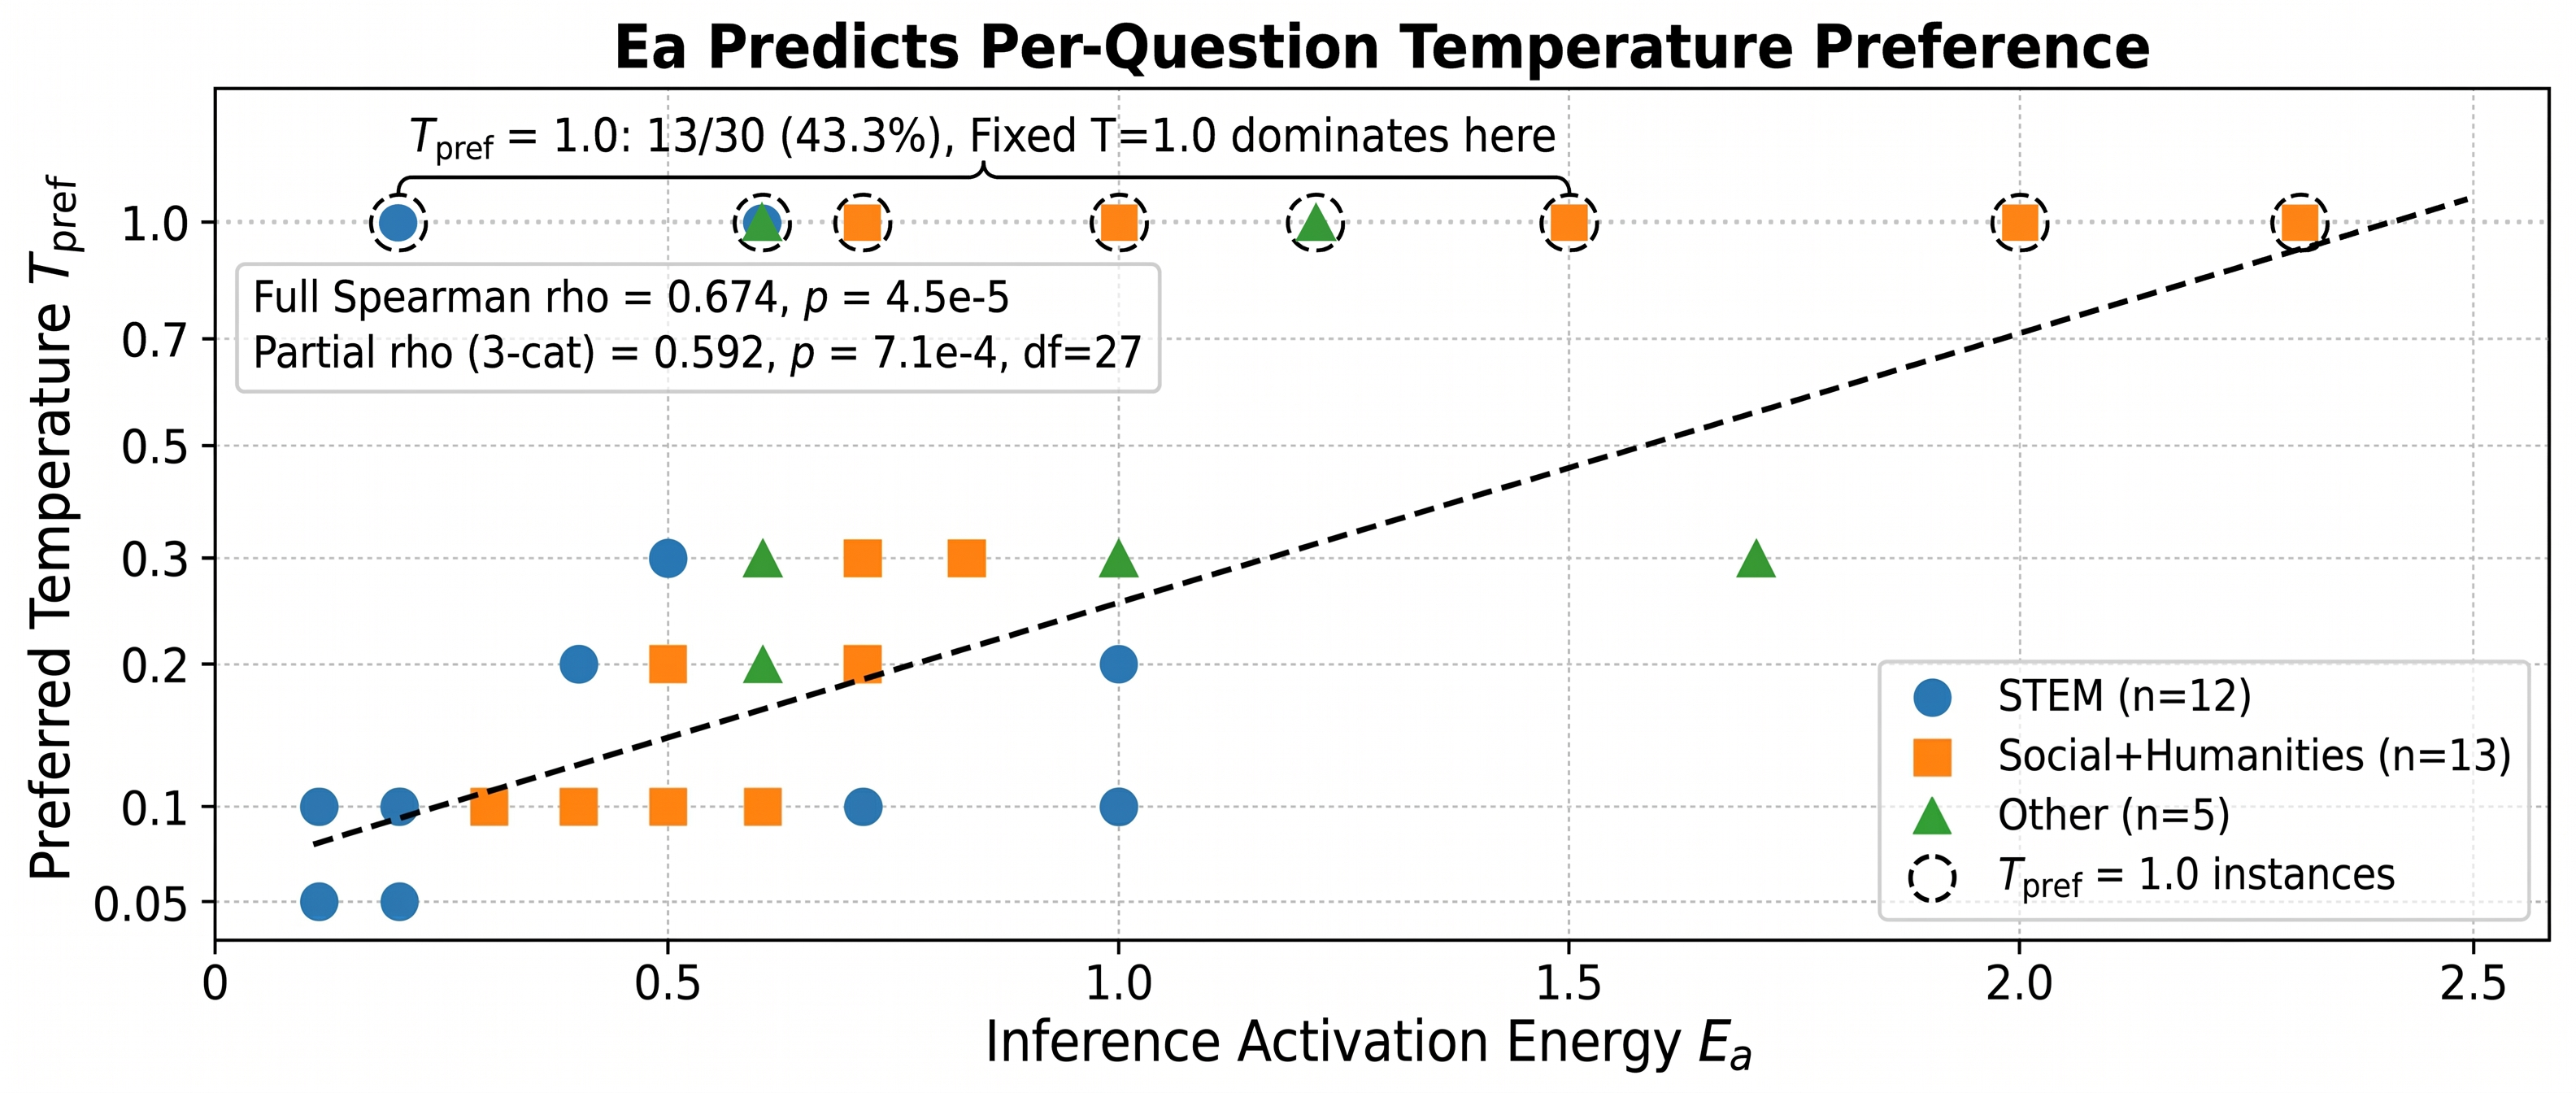
\includegraphics[width=\textwidth,height=0.45\textheight,keepaspectratio]{figures/fig5_v0.jpg}
  \caption{Scatter plot of inference activation energy $E_a$ versus empirically preferred
  temperature $T_\text{pref}$ for 30 valid phi-4/MMLU-Pro instances, colored by collapsed
  subject category (STEM: 12 instances, Social+Humanities: 13 instances, Other: 5
  instances). Spearman $\rho = 0.674$ ($p = 4.5 \times 10^{-5}$); collapsed 3-category
  partial Spearman $\rho_\text{partial} = 0.592$ ($p = 7.1 \times 10^{-4}$, df $= 27$).
  The 13 instances with $T_\text{pref} = 1.0$ (43.3\%) are shown with dashed outlines; on
  these instances, Fixed $T=1.0$ achieves 100\% accuracy while $T_\text{operating}$
  achieves 84.6\%.}
  \label{fig:ea-tpref}
\end{figure*}

\subsection{Model-Class Sensitivity}

\textbf{Ministral-8B.} A secondary experiment on mistralai/ministral-8b-2512 (\$0.485)
yielded $n=7$ valid Arrhenius fits (underpowered).%
\footnote{Code: \url{https://github.com/AMGrobelnik/ai-invention-ce2af9-arrhenius-kinetics-of-llm-inference-acti/tree/main/round-4/experiment-1}}
Median $R^2 = 0.382$ (bootstrap 95\% CI: $[0.158, 0.551]$), far below phi-4's 0.848. The
mechanistic interpretation: median $E_a = 0.085$ (vs.\ phi-4's 0.351). When logit gaps
are small, the Arrhenius regression has poor signal-to-noise ratio, producing low $R^2$
regardless of model architecture. The relevant model-class predictor is $E_a$ magnitude,
not model size.

\textbf{Cross-benchmark pattern.} Table~\ref{tab:crossbench} summarizes the three
experimental conditions.

\begin{table}[!htbp]
\centering
\caption{Comparison across experimental conditions. Two-token dominance (TD) is confirmed
only on ARC-Challenge $K=4$, where $\rho(E_a, \Delta)=0.936$. Valid-fit rate is primarily
predicted by $E_a$ magnitude and $K$.}
\label{tab:crossbench}
\small
\begin{tabular}{llllll}
\hline
Condition & $K$ & Med.\ $E_a$ & $\rho(E_a,\Delta)$ & Fit\% & Med.\ $R^2$ \\
\hline
MMLU-Pro & 10 (phi-4) & 0.351 & 0.106 & 19.9 & 0.848 \\
MMLU-Pro & 10 (Min-8B) & 0.085 & 0.0 & 6.9 & 0.382 \\
ARC-Ch.  & 4  (phi-4) & 0.393 & \textbf{0.936} & \textbf{54} & 0.871 \\
\hline
\end{tabular}
\end{table}

The cross-benchmark pattern identifies two distinct failure modes: (1) mass diffusion
(large $K$, many competing options) degrades two-token dominance and reduces valid-fit
rate; (2) small $E_a$ (low logit gaps) degrades fit quality regardless of $K$. The
ARC-Challenge result indicates that two-token dominance is recoverable by reducing $K$,
and that the Arrhenius framework may work well in practice for MCQA tasks with fewer
answer options.

%% ============================================================
\section{Related Work}
%% ============================================================

\textbf{Softmax-Boltzmann equivalence.} Bridle~\cite{Bridle1989} introduced the
normalised exponential for probabilistic neural network outputs; Hinton et al.~\cite{Hinton2015}
formalized the temperature-scaled variant for knowledge distillation. Luce's choice axiom
(1959) independently derives the same functional form. Our contribution is not the
Arrhenius-softmax equivalence (which follows directly from the Gibbs distribution
correspondence) but the threshold temperature formula $T_\text{thresh} = E_a/\ln N$, its
Lean~4 formal verification, and its empirical validation as a mechanistic predictor of
per-instance temperature preference.

\textbf{Per-question temperature heterogeneity.} Wu et al.~\cite{Wu2025} show per-question
preferred temperature varies substantially across questions on Qwen3 models, with
multi-temperature scaling yielding $+7.3$ pp over single-temperature protocols on hard
reasoning benchmarks. Their protocol requires 1,024 samples per temperature across 13
temperatures---13,312 forward passes per question---and their entropy analysis fails for
hard questions. The Arrhenius $E_a$ explains 45.4\% of per-question temperature variance
in our experiment ($\rho = 0.674$, $n=30$) from a temperature sweep without generating
any reasoning traces.

\textbf{Dataset-level temperature optimization.} Du et al.~\cite{Du2025} (TURN, ICML 2025)
identify the entropy turning point $T_\text{TURN}^\text{emp}$ as an automated
dataset-level upper bound on useful temperature. The present paper introduces an explicit
notation distinguishing $T_\text{TURN}^\text{emp}$ (Du et al.'s empirical quantity,
median 1.4 on phi-4) from $T_\text{TURN}^\text{theory} = E_a/\ln K$ (the theoretical
bound in Theorem~6, median 0.153), which differ by approximately $9\times$ on
phi-4/MMLU-Pro. These quantities are complementary: $T_\text{TURN}^\text{theory}$ bounds
each instance individually; $T_\text{TURN}^\text{emp}$ averages across the dataset.

\textbf{Temperature recalibration.} Guo et al.~\cite{Guo2025} (SMART, 2025) derive a
recalibration bound for achieving a target confidence $\hat{p}$ from the logit gap between
the argmax token and the second-highest token. The logit gap in SMART is
argmax-vs-second regardless of whether the argmax is correct; $E_a$ in the Arrhenius
framework is specifically the correct-vs-wrong gap in the OC regime. The two methods
address complementary problems: SMART calibrates to a target confidence; $T_\text{thresh}$
selects the minimum temperature to recover a suppressed correct answer.

\textbf{Calibrated sampling.} Tang et al.~\cite{Tang2025} (CarBoN) learn per-input logit
adjustments to guide generation toward high-reward paths, achieving up to $4\times$
compute reduction. CarBoN requires an exploration phase; $T_\text{thresh}$ requires a
temperature sweep. The approaches are complementary: $T_\text{thresh}$ identifies the
operating temperature window, and CarBoN could calibrate generation within that window.

\textbf{Logit-gap diagnostics.} Li and Liu~\cite{Li2025} use the refusal-affirmation
logit gap as a one-pass diagnostic for alignment robustness. The mechanism---using a logit
gap between competing tokens as a diagnostic---parallels the $\Delta$ measurement in this
work, applied to safety rather than temperature selection.

\textbf{MCQA at scale.} Renze and Guven~\cite{Renze2024} confirm no statistically
significant aggregate temperature effect on MCQA accuracy across $T \in [0, 1.0]$,
consistent with the Arrhenius framework: the rising-limb signal exists only in the OC
subset identified by the pilot gate. Medical licensing exams (MedQA~\cite{Jin2020};
12,723 USMLE questions) and MMLU~\cite{Hendrycks2020} represent practical applied-domain
MCQA settings where per-instance temperature calibration is practically relevant.

%% ============================================================
\section{Discussion}
%% ============================================================

\subsection{Interpreting the Results}

The experiment produces a clear three-way dissociation. \emph{Structural predictions}---$T_\text{thresh}$
as a reliable lower bound and $E_a$ as a mechanistic predictor of per-question temperature
preference---are confirmed with adequate statistical power. \emph{Approximation accuracy}---that
a single logprob call ($\Delta$) suffices as a proxy for the regression ($E_a$)---fails
for phi-4/MMLU-Pro ($\rho(E_a, \Delta) = 0.106$) but holds on ARC-Challenge ($\rho(E_a,
\Delta) = 0.936$). \emph{Accuracy improvement}---that $T_\text{operating}$ outperforms
the simplest zero-cost baseline, Fixed $T=1.0$---is not confirmed ($-3.3$ pp; McNemar
$p=0.500$; all CIs overlapping).

The accuracy result has a precise mechanistic explanation in the subgroup analysis. With
43.3\% of valid instances having $T_\text{pref} = 1.0$, and median $T_\text{operating}
\approx 0.43$, the framework systematically undershoots the preferred temperature for the
most common subgroup. Fixed $T=1.0$ correctly handles this majority by construction. For
the 56.7\% with $T_\text{pref} < 1.0$---where differentiation is possible and the
framework provides genuine insight---both strategies achieve 88.2\%, and $n=17$ is
insufficient to discriminate. Confirming an advantage in this subgroup requires
approximately $n \geq 200$ valid instances with $T_\text{pref} < 1.0$.

The ARC-Challenge result changes the interpretation of the $\rho(E_a, \Delta)$ failure
on MMLU-Pro. That failure is not a fundamental limitation of the Arrhenius framework but
a dataset-specific consequence of the large number of competing answer options ($K=10$).
With $K=4$, the single-call approximation holds near-perfectly, and the valid-fit rate
more than doubles.

\subsection{Practical Deployment Algorithm}

The framework is scoped to MCQA tasks with unambiguous single-token correct and wrong
answers. The routing algorithm follows from the experimental findings:

\textbf{Algorithm~1: Arrhenius Temperature Routing.}
\begin{enumerate}[leftmargin=*,topsep=2pt,itemsep=2pt]
  \item \emph{Greedy check:} Run greedy decoding at $T = 0$. If correct, return directly
  (approximately 66\% of phi-4 MMLU-Pro examples).
  \item \emph{OC detection:} Extract $\text{logprob}(\text{correct token})$ at $T=1$. If
  $\text{logprob} < -10$ (approximately zero logit mass), fall back to Fixed $T=1.0$
  (approximately 27\% of phi-4 MMLU-Pro examples).
  \item \emph{Calibration check:} If a calibration set (50 instances) confirms $\rho(E_a,
  \Delta) \geq 0.6$ and $\text{CV}(\log A) < 0.4$ (as on ARC-Challenge $K=4$): compute
  $T_\text{thresh,approx} = \Delta/\ln N$ from the single logprob call. Otherwise: run the
  350-sample Arrhenius regression to estimate $E_a$ and compute $T_\text{thresh} =
  E_a/\ln N$.
  \item \emph{Temperature selection:} Set $T_\text{operating} = T_\text{thresh} + 0.3$.
  \item \emph{Best-of-$N$ sampling:} Sample $N=16$ outputs at $T_\text{operating}$ and
  return the majority answer.
\end{enumerate}

On phi-4/MMLU-Pro, the framework applies to approximately 6.7\% of examples (30/151 OC
instances with valid fits from 450 main-set items). On ARC-Challenge ($K=4$), the
applicable fraction rises to approximately 6.9\%, but with substantially stronger
$E_a$--$\Delta$ correspondence enabling the single-call approximation. For the mass-diffusion
regime (large $K$, $\rho(E_a, \Delta) < 0.3$), Fixed $T=1.0$ is a stronger practical
choice and should be used instead.

\subsection{Future Work}

\textbf{Target model class.} The hypothesis predicts that models with 55--75\% MMLU-Pro
baseline accuracy and moderately concentrated logit distributions (median $E_a \geq 0.2$)
will show both higher valid-fit rates and stronger two-token dominance than phi-4 on
MMLU-Pro. Testing this prediction on a mid-accuracy model with $n \geq 200$ valid
instances would power the accuracy comparison and validate the efficiency tradeoff of the
single-call approximation.

\textbf{CoT catalysis.} Chain-of-thought (CoT) prompting may act as a kinetic catalyst
by raising the correct token's logit rather than solely suppressing the wrong token's
logit. A test with $n \geq 50$ valid instance pairs under zero-shot vs.\ CoT
conditions---measuring $\Delta l_c$ and $\Delta l_w$ separately---would determine whether
the dominant mechanism is catalytic (raising $l_c$) or re-ranking (lowering $l_w$). The
current evidence ($n=3$ valid pairs in the catalysis test) is insufficient for any
conclusion.

\textbf{Multi-token generation.} Extending the Arrhenius framework to sequence-level
generation requires measuring $P(\text{correct sequence}|T)$ rather than a single-token
logprob, which demands a different protocol and reference distribution. The single-token
formalism developed here provides a clean starting point.

\subsection{Limitations}

\textbf{Statistical power.} The accuracy comparison (C7) is underpowered at $n=30$; all
CP intervals overlap. The $E_a$--$T_\text{pref}$ correlation (C6) is well-powered
(observed $\rho = 0.674 \gg$ minimum detectable $\rho \approx 0.492$). Future work
should target $n \geq 100$ valid instances for structural predictions and $n \geq 200$
for accuracy comparisons.

\textbf{Model dependence.} Two-token dominance fails for phi-4 on MMLU-Pro (mass
diffusion, 10 competing options) and is not confirmed for Ministral-8B (small $E_a =
0.085$). The ARC-Challenge experiment shows two-token dominance recovers with $K=4$, but
$\text{CV}(\log A)$ remains above the strict threshold.

\textbf{Low valid-fit fraction on MMLU-Pro.} Only 19.9\% of phi-4 OC instances exhibit
temperature sensitivity in $[0.05, 1.0]$, consistent with the pilot gate failure (14\%
rising fraction). Models with lower MMLU-Pro accuracy---more errors, more cases where the
correct token has appreciable but suppressed logit mass---would increase this substantially.

\textbf{Pre-specified criteria.} Nine empirical criteria were pre-specified in pipeline
planning artifacts prior to running the main experiment. These are reported as
pre-specified rather than formally pre-registered (no public registry was used);
independent verification of criterion precedence requires inspection of artifact timestamps
in the pipeline repository.

\textbf{MCQA-only scope.} All quantitative results are restricted to single-token MCQA.
Extension to multi-token generation requires a different measurement protocol.

%% ============================================================
\section{Conclusion}
%% ============================================================

We derive, formally verify (10 Lean~4 theorems, \texttt{sorry}-free), and empirically
test the Arrhenius inference framework for per-instance temperature selection in MCQA.
The central empirical finding is that $E_a$ explains 45.4\% of per-question temperature
preference variance ($\rho = 0.674$, $p = 4.5 \times 10^{-5}$, $n=30$; partial $\rho =
0.592$, $p = 7.1 \times 10^{-4}$, df$=27$ with collapsed 3-category subject control),
providing a mechanistic predictor of the question-level heterogeneity documented by Wu et
al.~\cite{Wu2025}. Three results are explicit from the evidence: (1) the routing strategy
$T_\text{operating}$ does not outperform Fixed $T=1.0$ on phi-4/MMLU-Pro within
statistical precision (McNemar $p=0.500$; Fixed $T=1.0$ is the stronger zero-cost
baseline); (2) two-token dominance fails for phi-4 on MMLU-Pro ($K=10$) but holds on
ARC-Challenge ($K=4$, $\rho(E_a, \Delta) = 0.936$), isolating the answer-option count
as the operative mechanism; (3) the valid-fit rate rises from 19.9\% to 54\% when $K$
decreases from 10 to 4, pointing to a concrete path toward making the single-call
approximation practical. Future work targeting mid-accuracy models with $n \geq 200$
valid instances from $K \leq 4$ benchmarks is well-positioned to confirm a statistically
detectable accuracy advantage.

\bibliographystyle{unsrtnat}
\bibliography{references}

\end{document}
